%% BioMed_Central_Tex_Template_v1.06
%%                                      %
%  bmc_article.tex            ver: 1.06 %
%                                       %

%%IMPORTANT: do not delete the first line of this template
%%It must be present to enable the BMC Submission system to
%%recognise this template!!

%%%%%%%%%%%%%%%%%%%%%%%%%%%%%%%%%%%%%%%%%
%%                                     %%
%%  LaTeX template for BioMed Central  %%
%%     journal article submissions     %%
%%                                     %%
%%          <8 June 2012>              %%
%%                                     %%
%%                                     %%
%%%%%%%%%%%%%%%%%%%%%%%%%%%%%%%%%%%%%%%%%


%%%%%%%%%%%%%%%%%%%%%%%%%%%%%%%%%%%%%%%%%%%%%%%%%%%%%%%%%%%%%%%%%%%%%
%%                                                                 %%
%% For instructions on how to fill out this Tex template           %%
%% document please refer to Readme.html and the instructions for   %%
%% authors page on the biomed central website                      %%
%% http://www.biomedcentral.com/info/authors/                      %%
%%                                                                 %%
%% Please do not use \input{...} to include other tex files.       %%
%% Submit your LaTeX manuscript as one .tex document.              %%
%%                                                                 %%
%% All additional figures and files should be attached             %%
%% separately and not embedded in the \TeX\ document itself.       %%
%%                                                                 %%
%% BioMed Central currently use the MikTex distribution of         %%
%% TeX for Windows) of TeX and LaTeX.  This is available from      %%
%% http://www.miktex.org                                           %%
%%                                                                 %%
%%%%%%%%%%%%%%%%%%%%%%%%%%%%%%%%%%%%%%%%%%%%%%%%%%%%%%%%%%%%%%%%%%%%%

%%% additional documentclass options:
%  [doublespacing]
%  [linenumbers]   - put the line numbers on margins

%%% loading packages, author definitions

\documentclass[twocolumn]{bmcart}% uncomment this for twocolumn layout and comment line below
%\documentclass{bmcart}

%%% Load packages
%\usepackage{amsthm,amsmath}
%\RequirePackage{natbib}
%\RequirePackage{hyperref}
\usepackage[utf8]{inputenc} %unicode support
%\usepackage[applemac]{inputenc} %applemac support if unicode package fails
%\usepackage[latin1]{inputenc} %UNIX support if unicode package fails
\usepackage{graphicx}

%%%%%%%%%%%%%%%%%%%%%%%%%%%%%%%%%%%%%%%%%%%%%%%%%
%%                                             %%
%%  If you wish to display your graphics for   %%
%%  your own use using includegraphic or       %%
%%  includegraphics, then comment out the      %%
%%  following two lines of code.               %%
%%  NB: These line *must* be included when     %%
%%  submitting to BMC.                         %%
%%  All figure files must be submitted as      %%
%%  separate graphics through the BMC          %%
%%  submission process, not included in the    %%
%%  submitted article.                         %%
%%                                             %%
%%%%%%%%%%%%%%%%%%%%%%%%%%%%%%%%%%%%%%%%%%%%%%%%%


%\def\includegraphic{figures/Features.pdf}
%\def\includegraphics{}



%%% Put your definitions there:
\startlocaldefs
\endlocaldefs


%%% Begin ...
\begin{document}

%%% Start of article front matter
\begin{frontmatter}

\begin{fmbox}
\dochead{Software}

%%%%%%%%%%%%%%%%%%%%%%%%%%%%%%%%%%%%%%%%%%%%%%
%%                                          %%
%% Enter the title of your article here     %%
%%                                          %%
%%%%%%%%%%%%%%%%%%%%%%%%%%%%%%%%%%%%%%%%%%%%%%

\title{GenNet: A Tool for Qualitative and Quantitative Modelling of Gene Regulatory Networks}

%%%%%%%%%%%%%%%%%%%%%%%%%%%%%%%%%%%%%%%%%%%%%%
%%                                          %%
%% Enter the authors here                   %%
%%                                          %%
%% Specify information, if available,       %%
%% in the form:                             %%
%%   <key>={<id1>,<id2>}                    %%
%%   <key>=                                 %%
%% Comment or delete the keys which are     %%
%% not used. Repeat \author command as much %%
%% as required.                             %%
%%                                          %%
%%%%%%%%%%%%%%%%%%%%%%%%%%%%%%%%%%%%%%%%%%%%%%

\author[
   addressref={aff1},                   % id's of addresses, e.g. {aff1,aff2}
   corref={aff1},                       % id of corresponding address, if any
   noteref={n1},                        % id's of article notes, if any
   email={leepianz@gmail.com}   % email address
]{\inits{SSG}\fnm{Syed Sabah-ud-din} \snm{Gilani}}
%\author[
 %  addressref={aff2},
  % corref={aff1},  
   %email={jamil.ahmad@gmail.com}
%]{\inits{JA}\fnm{Jamil} \snm{Ahmad}}

%\author[
%   addressref={aff3},
%   email={leepianz@gmail.com}
%]{\inits{TS}\fnm{Tariq} \snm{Saeed}}

%%%%%%%%%%%%%%%%%%%%%%%%%%%%%%%%%%%%%%%%%%%%%%
%%                                          %%
%% Enter the authors' addresses here        %%
%%                                          %%
%% Repeat \address commands as much as      %%
%% required.                                %%
%%                                          %%
%%%%%%%%%%%%%%%%%%%%%%%%%%%%%%%%%%%%%%%%%%%%%%

\address[id=aff1]{%                           % unique id
  \orgname{Research Center for Modelling and Simulation (RCMS), NUST}, % university, etc
  \street{Sector H-12},                     %
  \postcode{44000}                                % post or zip code
  \city{Islamabad},                              % city
  \cny{Pakistan}                                    % country
}
\address[id=aff2]{%
  \orgname{Research Center for Modelling and Simulation (RCMS), NUST},
  \street{Sector H-12},
  \postcode{44000}
  \city{Islamabad},
  \cny{Pakistan}
}

\address[id=aff3]{%
  \orgname{Research Center for Modelling and Simulation (RCMS), NUST},
  \street{Sector H-12},
  \postcode{44000}
  \city{Islamabad},
  \cny{Pakistan}
}

%%%%%%%%%%%%%%%%%%%%%%%%%%%%%%%%%%%%%%%%%%%%%%
%%                                          %%
%% Enter short notes here                   %%
%%                                          %%
%% Short notes will be after addresses      %%
%% on first page.                           %%
%%                                          %%
%%%%%%%%%%%%%%%%%%%%%%%%%%%%%%%%%%%%%%%%%%%%%%

\begin{artnotes}
%\note{About Author}     % note to the article
\note[id=n1]{Author GenNet, MS Research Project} % note, connected to author
\end{artnotes}

%\end{fmbox}% comment this for two column layout

%%%%%%%%%%%%%%%%%%%%%%%%%%%%%%%%%%%%%%%%%%%%%%
%%                                          %%
%% The Abstract begins here                 %%
%%                                          %%
%% Please refer to the Instructions for     %%
%% authors on http://www.biomedcentral.com  %%
%% and include the section headings         %%
%% accordingly for your article type.       %%
%%                                          %%
%%%%%%%%%%%%%%%%%%%%%%%%%%%%%%%%%%%%%%%%%%%%%%

\begin{abstractbox}

\begin{abstract} % abstract
\parttitle{Background} %if any
Gene regulatory networks have an important role to study the behaviour of genes. By analysing these Gene Regulatory Networks we can get the detailed information i.e. the occurrence of diseases by changing behaviour of GRNs. Many different approaches are used (i.e. qualitative modelling and hybrid modelling) and various tools (i.e. GenoTech, GINsim) have been developed to model and simulate gene regulatory networks. GenoTech allows the user to specify a GRN on Graphical User Interface (GUI) according to the asynchronous multivalued logical functions of René Thomas, and to simulate and/or analyse its qualitative dynamical behaviour. Rene\'  Thomas discrete modelling of gene regulatory network (GRN) \cite{GUY} is  a well known approach to study the dynamics of genes. It deals with some parameters which reflect the possible targets of trajectories. Those parameters are priory unknown. These un-known parameters are fetched using another model checking tool SMBioNet\cite{SMB}. SMBioNet produces all the possible parameters satisfying the given Computational Logic Tree (CTL) formula as input. This approach involving logical parameters and conditions also known as qualitative modelling of GRN. However, this approach neglects the time delays for a gene to pass from one level of expression to another one i.e. inhibition to activation and vice versa. To find out these time delays, another modelling tool HyTech\cite{HTK} is used to perform hybrid modelling of GRN.

\parttitle{Results} %if any
We have developed a Java based tool called GenNet http://asanian.com/gennet to facilitate the model checking user by providing a unique GUI layout for both qualitative and quantitative modelling of GRNs. As we discussed, three separate modelling tools are used for complete modelling and analysis of a GRN. This process is much lengthy and takes too much time. GenNet assists the modelling users by providing some extra features i.e. CTL editor, parameters filtering and input/output files management.

\parttitle{Conclusion} %if any
GenNet takes a GRN network as input and does all the rest of computations i.e. CTL verification, K-parameters generation, parameter implication to GRN, state graph, hybrid modelling and parameter filtration automatically. GenNet serves the user by computing the results within seconds that were taking hours and days of manual computation.
\end{abstract}

%%%%%%%%%%%%%%%%%%%%%%%%%%%%%%%%%%%%%%%%%%%%%%
%%                                          %%
%% The keywords begin here                  %%
%%                                          %%
%% Put each keyword in separate \kwd{}.     %%
%%                                          %%
%%%%%%%%%%%%%%%%%%%%%%%%%%%%%%%%%%%%%%%%%%%%%%

\begin{keyword}
\kwd{Qualitative modelling}
\kwd{Quantitative modelling}
\kwd{GRN Modelling and analysis}
\kwd{Hybrid Modelling}
\kwd{Time delays}
\kwd{CTL verification}
\end{keyword}

% MSC classifications codes, if any
%\begin{keyword}[class=AMS]
%\kwd[Primary ]{}
%\kwd{}
%\kwd[; secondary ]{}
%\end{keyword}

\end{abstractbox}
%
\end{fmbox}% uncomment this for twcolumn layout

\end{frontmatter}

%%%%%%%%%%%%%%%%%%%%%%%%%%%%%%%%%%%%%%%%%%%%%%
%%                                          %%
%% The Main Body begins here                %%
%%                                          %%
%% Please refer to the instructions for     %%
%% authors on:                              %%
%% http://www.biomedcentral.com/info/authors%%
%% and include the section headings         %%
%% accordingly for your article type.       %%
%%                                          %%
%% See the Results and Discussion section   %%
%% for details on how to create sub-sections%%
%%                                          %%
%% use \cite{...} to cite references        %%
%%  \cite{koon} and                         %%
%%  \cite{oreg,khar,zvai,xjon,schn,pond}    %%
%%  \nocite{smith,marg,hunn,advi,koha,mouse}%%
%%                                          %%
%%%%%%%%%%%%%%%%%%%%%%%%%%%%%%%%%%%%%%%%%%%%%%

%%%%%%%%%%%%%%%%%%%%%%%%% start of article main body
% <put your article body there>

%%%%%%%%%%%%%%%%
%% Background %%
%%
\section*{Background}
In any given cell, thousands of genes are expressed and work in concert to ensure the cell's function, fitness, and survival. Each gene, in turn, must be expressed at the proper time and in the proper amounts to ensure the appropriate functional outcome. The regulation and expression of some genes are highly robust; their expression is controlled by invariable expression programs. For instance, developmental gene expression is extremely similar in a given cell type from one individual to another. The expression of other genes is more variable: Their levels are noisy and are different from cell to cell and from individual to individual. This can be highly beneficial in physiological responses to outside cues and stresses. Recent advances have enabled the analysis of differential gene expression at a systems level. Gene regulatory networks (GRNs) involving interactions between large numbers of genes and their regulators have been mapped onto graphic diagrams that are used to visualize the regulatory relationships. Gene regulatory networks play very crucial role to study the behaviour of genes. Simulation and analysis of these Gene Regulatory Networks can leads a person to find out the detailed information i.e. the occurrence of diseases in the result of  changing behaviour of GRNs. Qualitative modeling and hybrid modeling are well known approaches to completely analyse these GRNs. There are so many tools (i.e. GenoTech, GINsim) developed for the modelling, simulation and analysis of these gene regulatory networks. 
\par GINsim allows the user to specify a GRN on Graphical User Interface (GUI) according to the asynchronous multivalued logical functions of René Thomas, and to simulate and/or analyse its qualitative dynamical behaviour. Rene\'  Thomas discrete modeling of gene regulatory network (GRN) \cite{GUY} is  a well known approach to study the dynamics of genes. It deals with some parameters which reflect the possible targets of trajectories. Those parameters are priory unknown. User have to manually enter these unknown parameters (K-parameters) in GINsim as because there is no feature in GINsim to find these K-parameters. These un-known parameters can be fetched using another model checking tool SMBioNet\cite{SMB} that uses NuSMV (a symbolic model checker). SMBioNet produces all the possible parameters satisfying the given Computational Logic Tree (CTL) formula as input but there is no facility to draw or load GRN in SMBioNet. GENOTECH also facilitates the user as GINsim with some extra features i.e. a good GUI interface but K-parameters are still fetched using SMBioNet. This approach involving logical parameters and conditions also known as qualitative modeling of GRN. However, this approach neglects the time delays for a gene to pass from one level of expression to another one i.e. the time to pass from inhibition to activation and vice versa. To find out these time delays, another modelling tool HyTech\cite{HTK} is used to perform hybrid modelling of GRN. However, HyTech is also a symbolic tool and there is no GUI.
\par As we discussed, the modelling and simulation of GRNs is very important but at the same time its too difficult and time taking because there is no single tool to completely analyse the system. At a minimum three separate modelling tools are used for complete modelling and analysis of a GRN. To remove this barrier and facilitate modelling users we propose GenNet, a tool to perform both qualitative and quantitative modelling of GRN under a single GUI interface. GenNet is capable of GRN editor, fetching K-parameters by verifying given CTL as well as hybrid modelling and analysis. Moreover, GenNet facilitates the modelling users by providing some extra features i.e. CTL editor, parameters filtering and input/output files management.

\section*{Implementation}
Figure 1 elucidates the layered architecture, upon which our implimentation is based. We use existing coed of SMBioNet and HyTech for parameter estimation and hybrid modeling of GRN respectively. These are shown in figure 1 as layer 2. In order to compute logical parameters, SMBioNet uses a model checker  NuSMv (shown as layer 3). On top of layer 2, we develop a Graphical User Interface (GUI) to access features of both SMBioNet and HyTech tools. For this purpose, we use the existing interface of GenoTech which uses a drag and drop model for construction of biological networks asa labelled directed graphs. We extend the existing interface of GenoTech by adding new features, which enable the user to build the SMBioNet model, directly from GenoTech graph. This alleviates the requirement to code SMNioNet input model separately. Moreover,, it facilitates by generating default logical parameters which can be modified by the user.
\begin{figure}[h!] 
  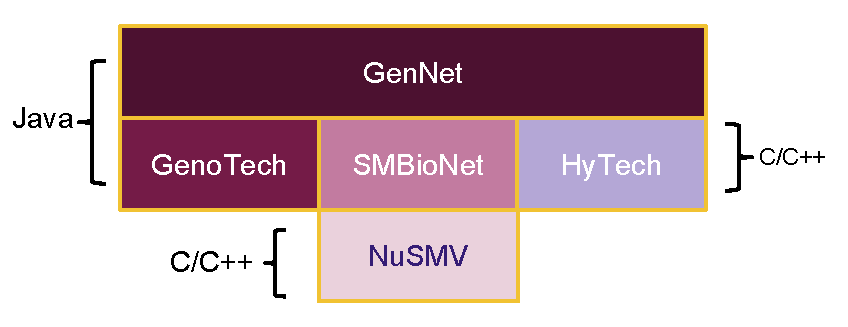
\includegraphics[scale=.55]{figures/Implementation.pdf}
  \caption{\csentence{Implementation.}
      GenNet implementation shows the layered architecture of the software.}
   
      \end{figure}

The entity relationship diagram (ERD) of our developed pipe-lined tool GenNet is shown as figure 2. In ERD, main interaction of tools with each other is shown where GenoTech deals with GRN, State graph and Hybrid Model generation. Pipe-Line Module forward the GRN file along with CTL (produced by GenoTech) to SMBioNet which further interacts with NuSMv model checker to verify the model. SMBioNet returns the output to Pipe-Line Module, where parser refines each parameter and sends back to GenoTech. Further, parameters are applied to GRN to generate the state graph and hybrid model as HyTech input.
\begin{figure*}[!ht] 
  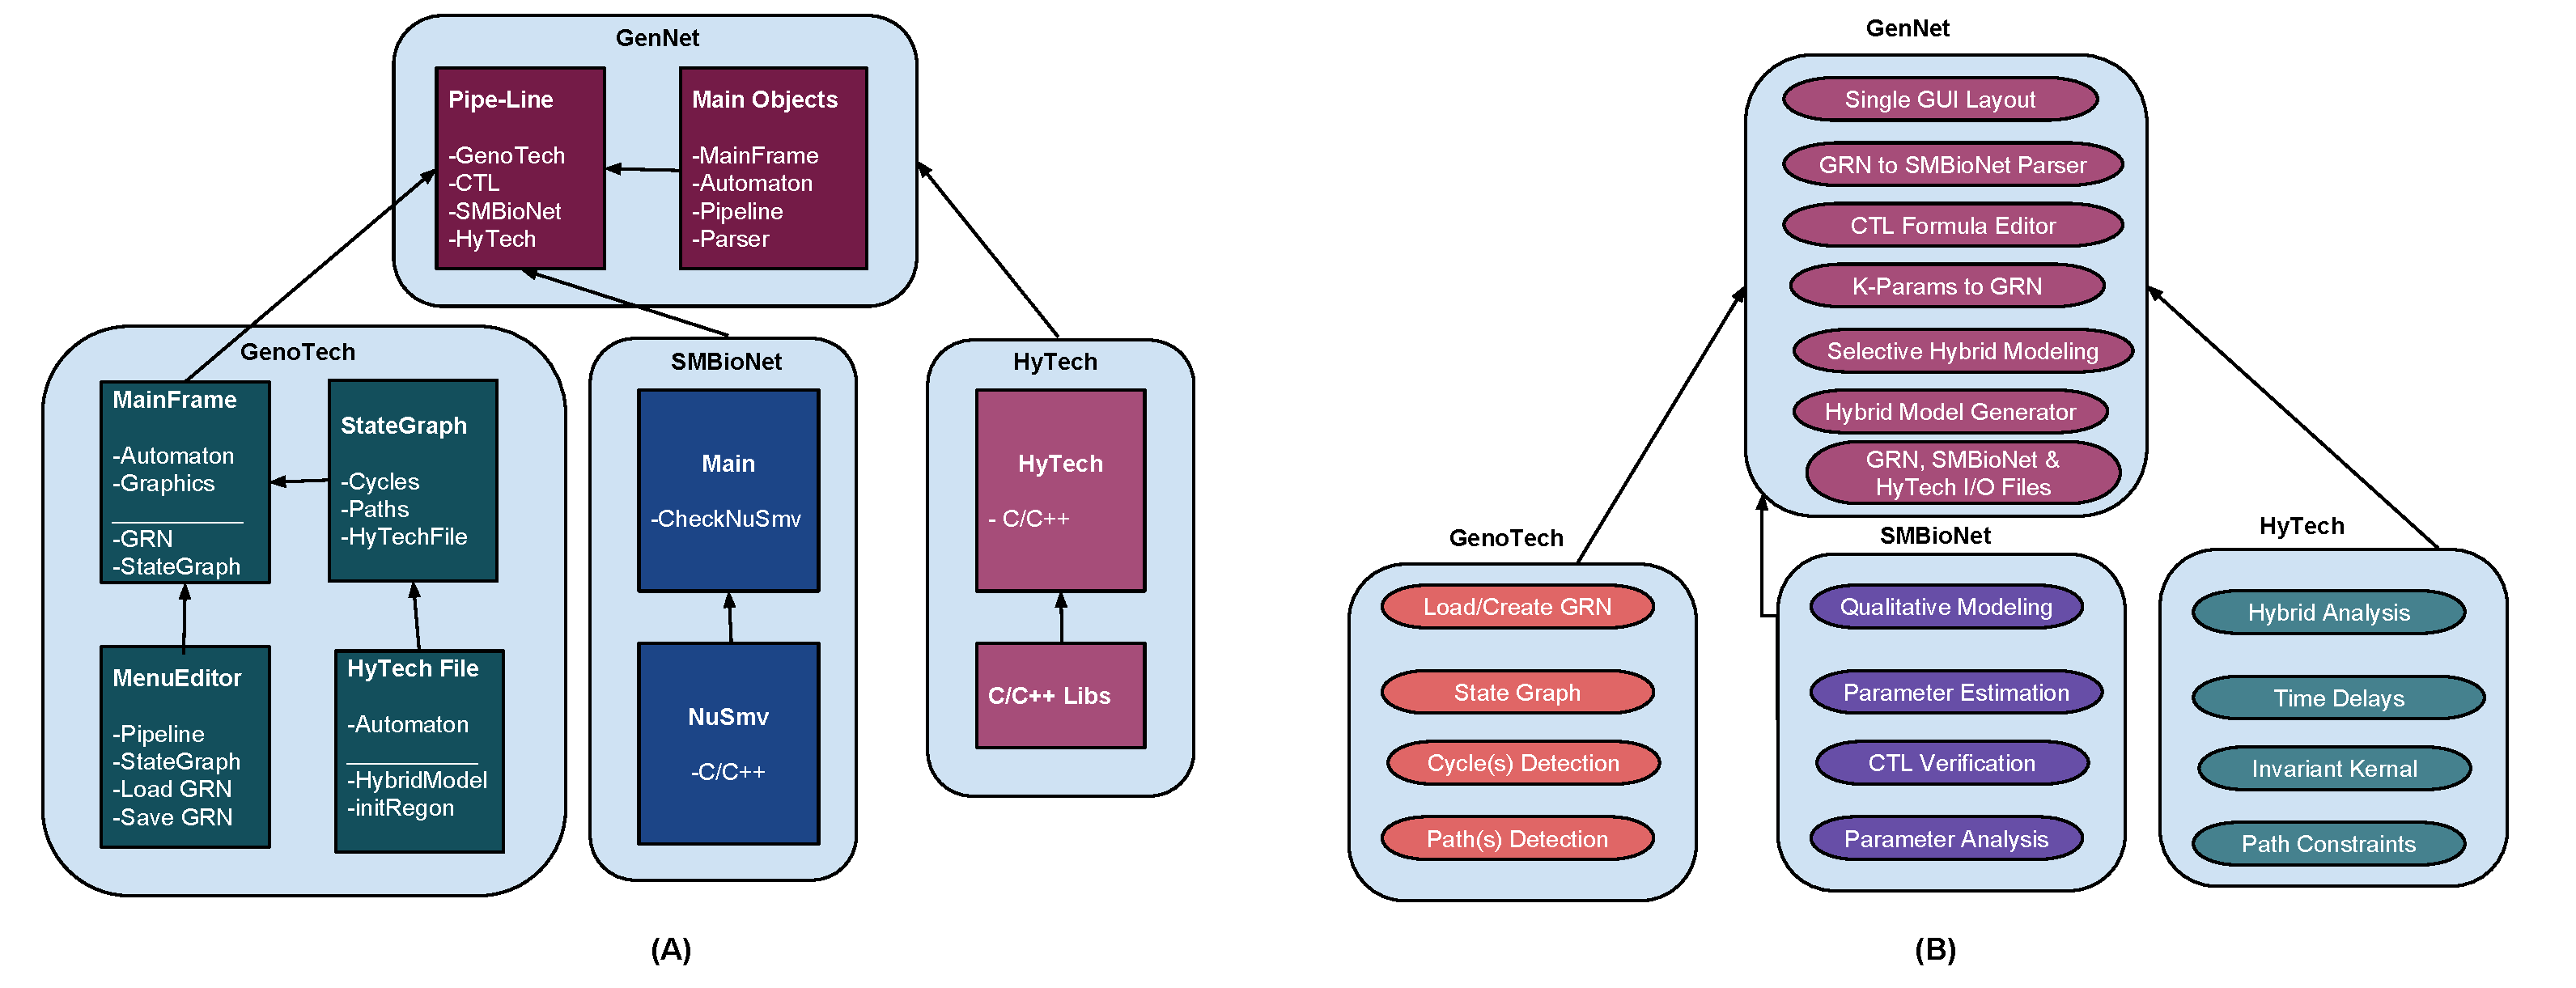
\includegraphics[scale=.31]{figures/ERD.pdf}
  \caption{\csentence{ERD.}
      (A) Entity relationship diagram shows the interaction between tools and their classes used. (B) Illustrates the main features of GenNet software tool.}
   
      \end{figure*}

The GenoTech models are by default stored as \emph{XML} objects. We used Java Document Object Model (DOM) to parse and extract requred information to generate its SMBioNet model.The CTL formula is provided by the user which is appended to SMBioNet input model using Java string library.
\\
The output of SMBioNet contains these set of logical parameters that satisfies the given CTL formula. This output is stored as a text file. We developed a parser that reads output produced by SMBioNet, and for eache parameter, it is possible to visualize its state graph along with important biological properties such as cycles, deadlock and importanct tragectories.
\\
We also develope a parser to parse all states to hybrid model, morover, we have implemented the technique to parse custome hybrid model in which user have options to select whether to generate hybrid model of specific cycle or complete state graph. This hybrid model is saved as text file which is available to user for further modifications. HyTech is used to verify the hybrid model and the output is shown on the same GUI fo GenoTech.
\\
Figure 3 shows the important features and capabilities of GenNet. Single GUI layout for GENOTECH, SMBioNet and HyTech provides very easy and fast modeling and analysis of biological regulatory networks (GRNs).GRN loaded or created by user parsed to SMBioNet input format and CTL formula editor is used to specify CTL logic which is further appended to SMBioNet iput file. Qualitative modeling and parameter estimation is performed using SMBioNet and selected models against specified CTL are shown as a list of parameter sets to user. User can select specific set of parameters which are directly applied to GRN model and the state graph is generated. User can view the Cycles, Deadlocks and nieghber states. Hybrid model can be generated from state graph, user have options to generate either hybrid model of complete state graph or a specific cycle. Also, user is facilitated to edit (can specify init-REG, initial loc etc) the generated hybrid model befor performing hybrid analysis using HyTech. HyTech output is also shown on Pip-Line GUI and user can find time delays, path constraints and inveriant kernal. The input and output files i.e. GRN, SMBioNet i/o files, Hybrid Model and result files are stored on disk so that user can reuse them.
%\begin{figure}[h!] 
  %\includegraphics[scale=.3]{figures/Features.pdf}
  %\caption{\csentence{Features.}
     % Illustrates the main features of GenNet software tool.}
   %
      %\end{figure}
      
      
Figure 4 illustrates the schematic architecture of GenNet. As shown in figure 4, the user interface of GenNet is capable of editing the loaded GRN as well as it is possible for the modelling user to create or design a new model using the GenNet editor. User interface module accepts GRN file as an XML and facilitates the user to analyse the GRN graph. It also provides the facility to add, edit and/or update the parameters to GRN network. GenNet parsers module contain GRN to XML parser that saves the GRN to XML and further parse that XML file to SMBioNet input file along with CTL formula. The parser module also parses the output of SMBioNet handled CTL verifier module. K-parameters are extracted from SMBioNet output and are arranged as an interactive sorted list for further use.
\par The specific model selected by user from K-parameters (extracted by parser module as discussed above) list is automatically applied back to GRN that leads the user to see state graph, cycles in the system and steady states. An interactive list of cycles occurring in the model is presented to the user. As shown in figure 4, the hybrid model generator module parses the state graph to generate HyTech hybrid model as '.hy' file. Hybrid model generator is capable of generating the complete hybrid model of the system or a specific cycle selected by user. The last but not the least module is Hybrid simulation, which passes the '.hy' file to HyTech and handles the output and present it to the user on GUI interface. Now, user can see hybrid results i.e. time delays, path constraints and invariant .  
\begin{figure*}[!ht] 
  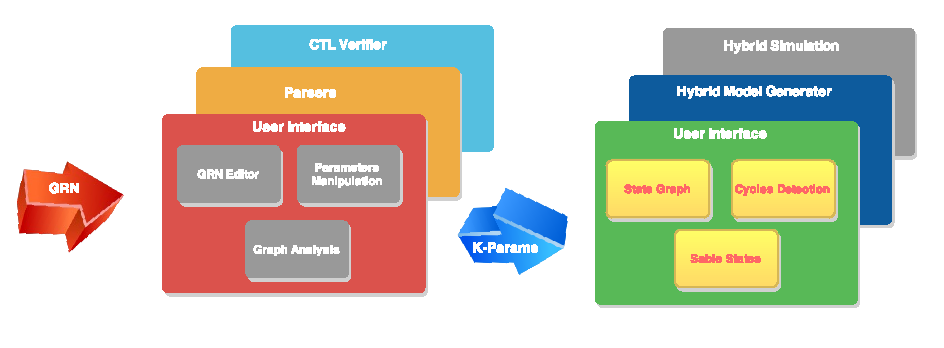
\includegraphics{figures/Arch.pdf}
  \caption{\csentence{Features.}
      Illustration of the schematic architecture of GenNet software tool.}
   
      \end{figure*} 

\section*{Results and Discussion}
We have applied many case studies i.e. Pseudomonous, MAL, DENV and Lambda Phage to GenNet for the testing, verification and performance analysis and comparison with other tool. In this section we will discus one of them and that is Lambda Phage. Lambda Phage is one of the most studied genetic regulatory networks. It controls immunity in temperate bacteriophage lambda which is a temperate virus. In this case, after infection due to bacterial population, many bacteria soon lyse and results to produce new phages. Some bacteria survive and carry lambda genome in a dormant form. The first response is called lytic and the second is lysogenic. In the lysogenic bacteria, viral DNA has integrated into the bacterial chromosome and will be faithfully transmitted to the bacterial progeny. In this condition, the
viral gene cI, produces a repressor which blocks the expression of all the other genes of the phage, thus making the viral genome harmless for the bacterium. Moreover, cI makes lysogenic bacteria immune towards other infections. Lysogenization necessitates two events, integration of the viral DNA into the bacterial chromosome and development of immunity due to the expression of the repressor. The choice between the lytic and lysogenic pathways is very similar to cell differentiation, in the sense that a given virus, infecting apparently
identical cells, can behave in two extremely different ways \cite[RCH].

\par The biological regulatory graph G of lambda phage is shown in figure 5 (A) which is designed using GenNet GUI editor. The GRN contains gene cI, cro, cII, and N which play an important role in regulation of immune control. Gene cI is activated by cII. After it get activated, gene cI remains ON because its product activates its own synthesis, but at the same time, gene cI switches off the other lambda genes, including cII which had just switched it on. In addition gene cro exerts a negative control on cI, directly and indirectly, by repressing gene cII. Finally, gene N exerts a positive control on cII and is itself under negative control of cI and cII. The variables cI, cro, cII and N leads to 48 possible states as their thresholds are 3, 4, 2 and 2 valued respectively.
\par When the viral genome integrates a cell, all the viral proteins are initially absent. Thus (0,0,0,0) corresponds to the initial state of the system. The existence of both responses, lytic and lysogenic, implies that there exist two paths starting from the initial state leading respectively to the lytic state and to the immune one. The lytic state is known to be characterized by high concentration of cro and a low concentration of cI, cII and N whereas immune state is characterized by high concentration of cI and low concentration of cro, cII and N. In [26], both states (0,2,0,0) and (0,3,0,0) correspond to the lytic state and (2,0,0,0) is the only state corresponding to the immunity. Without change of the environment, the choice between the lytic and the lysogenic pathways is irreversible, thus the lytic and immune states are steady. Then if the system reaches one state of the sets A={(0,2,0,0),(0,3,0,0)} or B={(2,0,0,0)}, then it will never leave it. These sets of states are said steady sets \cite[RCH].

\begin{figure*}[!ht] 
  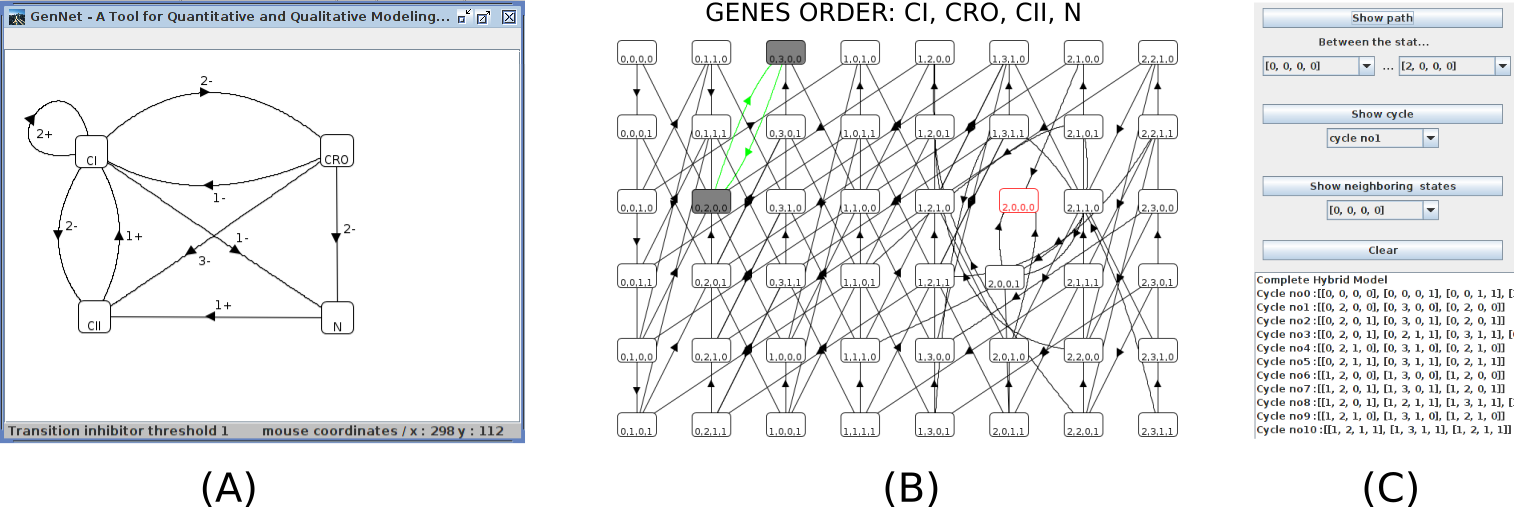
\includegraphics[scale=.38]{figures/GUI.png}
  \caption{\csentence{Features.}
      (A) GUI of GenNet with lambda phage GRN network. (B) State graph of GRN network. (C) Cycle detection, paths and hybrid model selection on GenNet GUI}
   
      \end{figure*}

\par There are 151200 total models returned by SMBioNet, out of which SMBioNet selects the 882 remaining models for the generated GRN verifying the CTL formula.
\par Figure 5 (B) show the state graph of the GRN model along with steady states. Although 4 positive feedback circuits are present in the regulatory graph, the selected models present only two steady states (regular or singular): (2,0,0,0) is always steady and the other one is either (0,2,0,0) or a singular state adjacent to (0,2,0,0) and (0,3,0,0). These steady states correspond to the lytic and immune states, and no other stable behavior (phenotype) can be observed. The steady state (2, 0, 0, 0) is highlighted in red and one can see that there are three incoming edges and no outgoing edge, so its a deadlock state. However, (0,2,0,0) and (0,3,0,0) is a single cycle highlighted with green edges.
\par GenNet facilitates the model checking user to select analyze individual cycle(s), path(s) and neighbor states as shown in Figure 5 (C). As Figure 5 (C) shows, there is a list of 11 cycles in the graph, these cycles can be selected individually to generate their hybrid model.
      
\section*{Conclusion}
Biological regulatory networks of any biological problem are very important to study and analyse. GenNet facilitates the user to completely simulate and analyse both qualitative and quantitative behaviours of GRNs. GenNet is Java base package easy to run and is user friendly where user especially biologists can define the problem easily. As compared with other tools available for modelling of GRNs, GenNet reduces the complexity and increases the performance by offering many extra features i.e. automatic K-parameters computation and implication, selective cycles in state graphs, hybrid modelling and analysis, result files backup and parameter filtration.
\section*{Availability and requirements}
\textbf{Project name:} GenNet
\\
\textbf{Project home page:} http://asanian.com/gennet
\\
\textbf{Operating system(s):} Linux
\\
\textbf{Programming language:} Java
\\
\textbf{Other requirements:} OpenJdk-7-jre
\\
\textbf{License:} GPL
\\
\textbf{Any restrictions to use by non-academics:} For commercial
use and modifications please contact the corresponding author.

%%%%%%%%%%%%%%%%%%%%%%%%%%%%%%%%%%%%%%%%%%%%%%
%%                                          %%
%% Backmatter begins here                   %%
%%                                          %%
%%%%%%%%%%%%%%%%%%%%%%%%%%%%%%%%%%%%%%%%%%%%%%

\begin{backmatter}

\section*{Competing interests}
  The authors declare that they have no competing interests.

\section*{Author's contributions}
  Gilani developed, designed, performed testing and analyses using different case studies. Gilani also wrote the paper and online help and support pages. Author read and approved the final manuscript.

\section*{Acknowledgements}
  Gilani is a National University of Science and Technology (NUST) MS Research Fellow. We thank the reviewers of this paper for their thoughtful comments.

%%%%%%%%%%%%%%%%%%%%%%%%%%%%%%%%%%%%%%%%%%%%%%%%%%%%%%%%%%%%%
%%                  The Bibliography                       %%
%%                                                         %%
%%  Bmc_mathpys.bst  will be used to                       %%
%%  create a .BBL file for submission.                     %%
%%  After submission of the .TEX file,                     %%
%%  you will be prompted to submit your .BBL file.         %%
%%                                                         %%
%%                                                         %%
%%  Note that the displayed Bibliography will not          %%
%%  necessarily be rendered by Latex exactly as specified  %%
%%  in the online Instructions for Authors.                %%
%%                                                         %%
%%%%%%%%%%%%%%%%%%%%%%%%%%%%%%%%%%%%%%%%%%%%%%%%%%%%%%%%%%%%%

% if your bibliography is in bibtex format, use those commands:
\bibliographystyle{bmc-mathphys} % Style BST file (bmc-mathphys, vancouver, spbasic).
\bibliography{bmc_article}      % Bibliography file (usually '*.bib' )

% or include bibliography directly:
% \begin{thebibliography}
% \bibitem{b1}
% \end{thebibliography}

%%%%%%%%%%%%%%%%%%%%%%%%%%%%%%%%%%%
%%                               %%
%% Figures                       %%
%%                               %%
%% NB: this is for captions and  %%
%% Titles. All graphics must be  %%
%% submitted separately and NOT  %%
%% included in the Tex document  %%
%%                               %%
%%%%%%%%%%%%%%%%%%%%%%%%%%%%%%%%%%%

%%
%% Do not use \listoffigures as most will included as separate files

%\section*{Figures}
 % \begin{figure}[!ht]
  %\caption{\csentence{Sample figure title.}}
   %   A short description of the figure content
    %  should go here.}
   
   % \fbox{\includegraphics[scale=.8]{Features.pdf}}
    
    %  \end{figure}

%\begin{figure}[h!]
 % \caption{\csentence{Sample figure title.}
  %    Figure legend text.}
   %   \end{figure}

%%%%%%%%%%%%%%%%%%%%%%%%%%%%%%%%%%%
%%                               %%
%% Tables                        %%
%%                               %%
%%%%%%%%%%%%%%%%%%%%%%%%%%%%%%%%%%%

%% Use of \listoftables is discouraged.
%%
%\section*{Tables}
%\begin{table}[h!]
%\caption{Sample table title. This is where the description of the table should go.}
 %     \begin{tabular}{cccc}
  %      \hline
   %        & B1  &B2   & B3\\ \hline
    %    A1 & 0.1 & 0.2 & 0.3\\
     %   A2 & ... & ..  & .\\
      %  A3 & ..  & .   & .\\ \hline
      %\end{tabular}
%\end{table}

%%%%%%%%%%%%%%%%%%%%%%%%%%%%%%%%%%%
%%                               %%
%% Additional Files              %%
%%                               %%
%%%%%%%%%%%%%%%%%%%%%%%%%%%%%%%%%%%

%\section*{Additional Files}
 % \subsection*{Additional file 1 --- Sample additional file title}
  %  Additional file descriptions text (including details of how to
   % view the file, if it is in a non-standard format or the file extension).  This might
%    refer to a multi-page table or a figure.

 % \subsection*{Additional file 2 --- Sample additional file title}
  %  Additional file descriptions text.


\end{backmatter}
\end{document}
